\chapter{Moléculas Fotónicas}

La técnica de escritura de guías de onda descrita en el capítulo \ref{cap:fs} está restringida por la forma alargada y elíptica del tren de pulsos láser que se enfoca, lo que en consecuencia constriñe los acoplamientos interorbitales posibles \citep{interorbital}. Una posibilidad para añadir grados de libertad es fabricar dos guías de onda lo suficientemente cercanas entre sí de manera de hibridizar sus modos guiados, de manera análoga al principio físico que rige a las moléculas. Es por ello que en este capítulo se usará el concepto de moléculas fotonicas \citep{molecules}, y su aplicación para el estudio experimental de una red fotónica que presenta una doble transición de fase topológica \citep{SPSSH}.

\section{Autoestados del acoplador fotónico para distancias de separación arbitrarias}

Como se adelantó en la sección \ref{cap:maxwell}, la teoría de modos acoplados es una buena descripción de los sistemas fotónicos en estudio siempre que la distancia de separación entre guías de onda sea superior a 15 $\mu$m, pues la constante de acoplamiento tiene un comportamiento exponencial decreciente. Más allá del régimen discreto, se hace necesario descibir el sistema como una sola macroguía. Una herramienta numérica que es agnóstica entre ambos regímenes es la de Expansión en Modos Normales, detallada en la sección \ref{cap:eme}. Es por ello que se simula un par de guías de onda a distintas distancias para determinar el comportamiento de sus autoestados. 

\section{Moléculas Fotónicas en Red SP-SSH}

Para la implementación experimental (sección \ref{cap:fs}) de una red que presente acoplamiento SP \citep{interorbital, SPSSH}, se utilizaron los dipolos horizontales de la sección anterior, obtenidos mediante moléculas fotónicas. Un preciso sintonizado de las constantes de propagación de los modos $s$ y $p$ permitió considerar un grado de libertad análogo al del espín del electrón (\textit{pseudoespín}). 

\begin{align*}
	H &= \sum_n \left[\delta\beta \left(- a^*_{n, 1} a_{n, 1} + b^*_{n, 1} b_{n, 1}  - a^*_{n, 2} a_{n, 2} + b^*_{n, 2} b_{n, 2}\right) +k_{ss, 2}a^*_{n, 2} a_{n, 1} -k_{pp, 2}b^*_{n, 2} b_{n, 1} \right. 
	\\	
	&\left. + k_{ss, 1} \left( a_{n-1, 2}^*a_{n, 1} + a_{n+1, 2}^*a_{n, 2} \right) - k_{pp, 1} \left( b_{n-1, 2}^*b_{n, 1} + b_{n+1, 2}^*b_{n, 2} \right) +k_{sp, 2} \left( a_{n, 2}^* b_{n, 1} - b_{n, 2}^* a_{n, 1} \right) \right]
\end{align*}

\begin{figure}[H]
\centering
	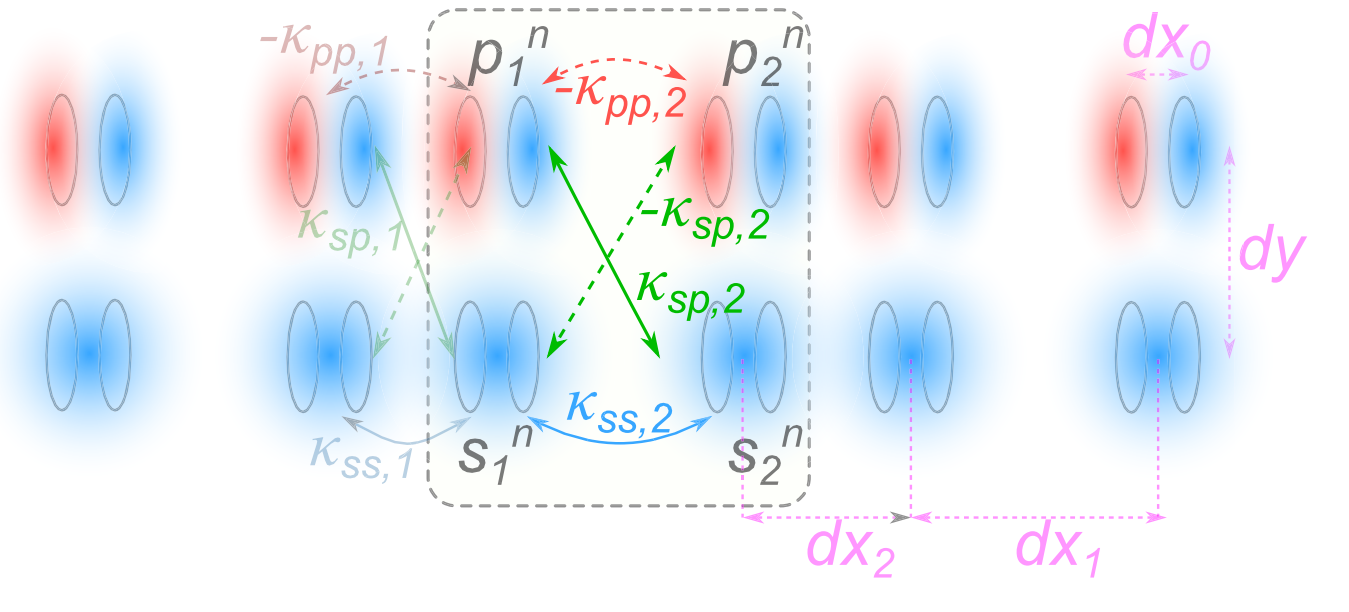
\includegraphics[width=0.7\linewidth]{media/ssh_sp_model}
	\caption{Esquema de la red SP-SSH}
\end{figure}